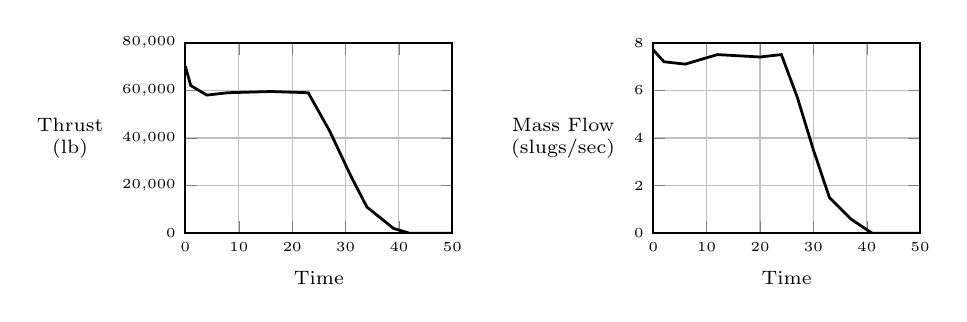
\begin{tikzpicture}
\begin{axis}[
  at={(0cm,0cm)},anchor=south west,
  width=0.41\linewidth,height=0.33\linewidth,
  xmin=0,xmax=50,ymin=0,ymax=80000,
  xtick={0,10,...,50},ytick={0,20000,...,80000},
  scaled y ticks=false,
  grid=major,
  xlabel={Time},ylabel={Thrust\\(lb)},
  ylabel style={align=center,rotate=-90},
  label style={font=\scriptsize},tick label style={font=\tiny},
  axis line style={line width=0.7pt}
]
\addplot[black,line width=1.0pt] coordinates {
  (0,70000) (1,62000) (4,58000) (8,59000) (16,59500) (23,59000)
  (27,43000) (31,24000) (34,11000) (39,2000) (42,0) (50,0)
};
\end{axis}
\begin{axis}[
  at={(0.49\linewidth,0cm)},anchor=south west,
  width=0.41\linewidth,height=0.33\linewidth,
  xmin=0,xmax=50,ymin=0,ymax=8,
  xtick={0,10,...,50},ytick={0,2,...,8},
  grid=major,
  xlabel={Time},ylabel={Mass Flow\\(slugs/sec)},
  ylabel style={align=center,rotate=-90},
  label style={font=\scriptsize},tick label style={font=\tiny},
  axis line style={line width=0.7pt}
]
\addplot[black,line width=1.0pt] coordinates {
  (0,7.7) (2,7.2) (6,7.1) (12,7.5) (20,7.4) (24,7.5)
  (27,5.7) (30,3.5) (33,1.5) (37,0.6) (41,0) (50,0)
};
\end{axis}
\end{tikzpicture}
